\documentclass[10pt, letter]{article}
\newcommand{\doctitle}{%
CS 4649/7649: RIP - Robot Intelligence - Planning}
\newcommand{\bigO}{\ensuremath{\mathcal{O}}}
\usepackage{graphicx}
\usepackage{float}
\usepackage{comment}
\usepackage{fancyvrb}
\usepackage{booktabs}
\usepackage[usenames,dvipsnames]{color}
\usepackage[center]{caption}
\usepackage{algorithm}
\usepackage[T1]{fontenc}
\usepackage[noend]{algpseudocode}
\usepackage{algorithm}
\usepackage[margin=1in]{geometry}
\usepackage[usenames,dvipsnames]{color}
\usepackage{hyperref}
\usepackage{xcolor}
\usepackage{amsmath}
\usepackage{subcaption}
\hypersetup{
  colorlinks,
  citecolor=Violet,
  linkcolor=Black,
  urlcolor=Blue}
%------------------------Included every possible package we might need ------------------------%
\begin{document}
\title{\textbf{\doctitle} \\\textsc{Project 1: Classical Sokoban Planner}}
  \author {Arvind Krishnaa Jagannathan, Zheng Yong, Luis Gustavo, Zhengyi Hu}%Others please check your names here
   \date{}
\maketitle

\section{Pre-Project: Towers of Hanoi}
%Assigned to Arvind%
\subsection*{Planners Used}
The two classical planners which we are using for the Towers of Hanoi problem are the Blackbox planner \cite{kautz1998blackbox} (downloaded from \url{http://www.cs.rochester.edu/~kautz/satplan/blackbox/blackbox-download.html}) and the FF planner \cite{hoffmann2001fast} (downloaded from \url{http://fai.cs.uni-saarland.de/hoffmann/ff/FF-v2.3.tgz}). The definition of the Towers of Hanoi domain, as well as the representation of the initial state of the problem (from Figure \ref{fig1}) are in the corresponding PDDL files, namely \textit{hanoi-domain.pddl} and \textit{hanoi-3.pddl}.

\begin{figure}[h!]
  \centering
    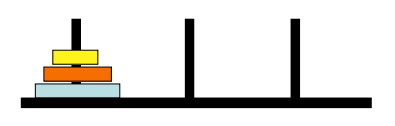
\includegraphics[scale = 0.3]{images/hanoi1}
    \caption{Towers of Hanoi with 3 disks}
  \label{fig1}
\end{figure}

\subsection{Questions}
\subsubsection*{1. Explain the method by which each of the two planners finds a solution}
\textbf{BlackBox}- The Blackbox planning algorithm essentially represents the PDDL representation of a problem as a set of Boolean satisfiability problems (SAT), which are then solved using a variety of SAT solvers (such as satz, walksat and chaff) to produce a plan.
In order to construct the SAT problem, Blackbox uses the \textsc{GraphPlan} algorithm to construct a plan graph for the given problem representation. This plan graph is then ``translated'' to the SAT problem representation. This is outlined briefly below:

The \textsc{GraphPlan} algorithm works by constructing a planning graph out of a \textsc{Strips} representation, which will propagate actions/operators across different ``layers'' along with their ``mutex'' pre-conditions. So at every stage there will be a list of actions, which have mutually exclusive pre-conditions. The plan generated by \textsc{GraphPlan} will be a sub-graph of the plan graph such that, all the conditions of the initial and final state are incorporated without there being any ``conflicting'' actions. As described by Kautz et. al \cite{kautz1996encoding}, each state in this solution graph can be encoded into propositional logic. This can be done by adding propositions of the form,
\begin{center}
$Precondition_i$ $\implies$ $Action_j$
\end{center}
At each layer of the solution sub-graph, clauses/fluents can be resolved away to result in a compact propositional logic representation of the plan graph. This list of proposition corresponds to the ``translation'' of the plan graph into a SAT problem. Then any available SAT solver can be applied on this problem which (although NP-complete in theory) with reasonable assumptions be completed in exponential time. ($O(n^3)$)

\textbf{FF Planner} - The fast-forward planning algorithm utilizes \textsc{GraphPlan} as an admissible (and informed) heuristic to solve the planning problem using a search algorithm across the set of permissible states in the state space. FF planner works as follows: it sets up a relaxed solvable sub-problem ($S\prime$) of the original problem ($S$).Then \textsc{GraphPlan} is applied on the relaxed sub-problem; the length of the solution plan sub-graph is then treated as a heuristic to guide the state space search algorithm for a plan to the original problem. This takes into account the positive interactions between various facts in the problem.

FF uses the enforced hill climbing algorithm to search for valid solutions. Using the length of the relaxed \textsc{GraphPlan} solution as a heuristic, the enforced hill climbing algorithm evaluates the direct successors of a search state S. Until a state ($S\prime$) is found with a better heuristic evaluation than $S$, the search goes one step further.

Thus in summary both \textit{\textbf{FF}} and \textit{\textbf{Blackbox}} algorithms use the \textsc{GraphPlan} algorithm, however \textit{Blackbox} uses it in a more direct way, to set up the SAT problem. In \textit{FF}, \textsc{GraphPlan} is used simply as a heuristic measure for the enforced hill climbing algorithm.
Both the planners generated the same plan, which is in Figure \ref{plan1}.

\begin{figure}[h!]
  \centering
    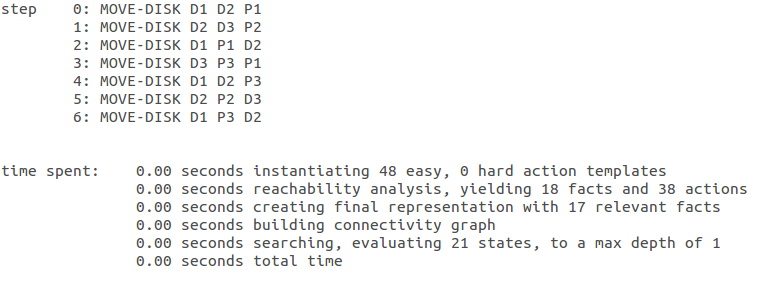
\includegraphics[scale = 0.5]{images/hanoi-3}
    \caption{Plan for Towers of Hanoi with 3 disks}
  \label{plan1}
\end{figure}

\subsubsection*{2. Which planner was fastest?}
\label{subsubsec_2}
Both the algorithms were run on the same Linux box, and using the \textit{time} command the time taken for them to produce plans were measure. Clearly the \textbf{FF} algorithm was the fastest among the two, with the following time measures \\
\begin{itemize}
\item FF - 0.004s
\item Blackbox - 0.011s
\end{itemize}
This shows that \textbf{FF} is 2.75 times faster than \textbf{Blackbox}. This is pretty much expected from theory since the time complexity for each of the algorithms are,
\begin{center}
	O(\textit{Blackbox}) = O(\textsc{GraphPlan'}) + O(\textit{SAT Solver})\\
	O(\textit{FF}) = O(\textsc{GraphPlan}) + O(\textit{Enforced Hill Climbing})\\
	O(\textit{Enforced Hill Climbing}) = O(iterations x successors),\\
	O(\textit{SAT Solver}) = O($2^n$)
\end{center}
Clearly the SAT solver's exponential time complexity, as well as the time complexity of the complete \textsc{GraphPlan} algorithm for \textit{Blackbox} vs. that of the relaxed \textsc{GraphPlan} as well as that of \textit{Enforced Hill Climbing} for the \textit{FF} make it obviously slower than FF; this has been shown by using the towers of hanoi state and domain PDDL description multiple times (to get an average measure) with Blackbox and FF.
\subsubsection*{3. Explain why the winning planner might be more effective on this problem}
Its pretty obvious that the length of a plan in case of the Towers of Hanoi problem are a similar order of magnitude as that of the total number of states ($2^n - 1$ steps and $3^n$ states). In case of the \textbf{FF} planner, \textsc{GraphPlan} is used only as a heuristic and that too for a relaxed subset. \textit{FF}'s major component is the local-search algorithm, which means it does not have to necessarily traverse all the states in order to obtain a solution.

\textit{Blackbox} on the other needs to explicitly construct the mutex graph for every level until a solution is obtained. In case the state space is large (like 10 disks in the Towers of Hanoi problem), the construction of a complete plan graph is memory prohibitive and will not be effective on larger instances of this problem (it actually does not give plans for even 6 disks on my machine after 1 minute of execution). Another major issue with \textit{Blackbox} is that several levels of the \textsc{GraphPlan} algorithm may lead to the same set of SAT problems, which will remain unsatisfiable. \textit{Blackbox} is bound to be less effective in similar large state problems, since it seems to perform the same computation multiple times.

%-----------------------------------End of Problem 1 ---------------------------------------------%

\section{Project Part I: Sokoban PDDL}
%Assigned to Luis%

\begin{figure}[h]
  \centering
    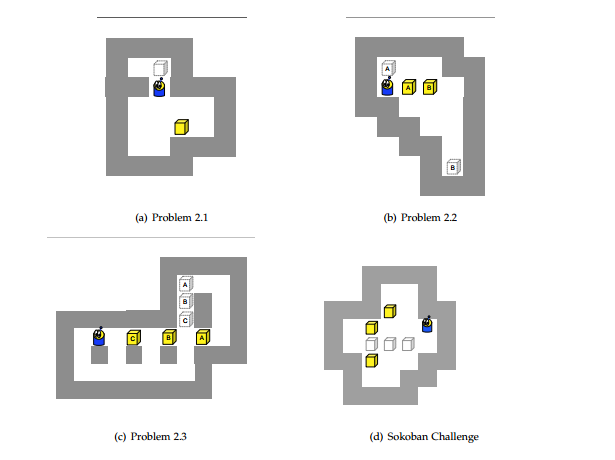
\includegraphics[scale = 0.5]{images/sokoban}
    \caption{Sokoban Problems}
  \label{fig2}
\end{figure}

\textbf{Note}: We have made the assumption that the \textit{planner can move any box to any target square}. This assumption is carried over to Part II as well.

The Sokoban's domain definition was created with the guideline idea of keeping it simple. Then, we followed the steps:

\begin{enumerate}
\item Identify the constants
\item Identify the fluents
\item Identify the actions
\end{enumerate} 

The first step is to identify the constants we evaluate possible elements that could be part of the domain. From this, constants like \textit{robot}, \textit{box} and \textit{location} appeared. However the problem only have one robot and is more natural to think about each box by its location instead of any kind of specific identification. Because of this, we moved on with only the \textit{location} constant.

The second step is to identify fluents related to this problem. We had a lot of possible fluents, most of them were related to the idea of using the constants already eliminated. However, to keep it simple, the fluents used were:

\begin{itemize}
\item \textbf{in(?loc)} - true if the robot is at location loc;
\item \textbf{boxAt(?loc)} - true if there is a box at location loc;
\item \textbf{isLeft(?loc ?loc)} - true if loc(1) is at left of loc(2);
\item \textbf{isRight(?loc ?loc)} - true if loc(1) is at right of loc(2);
\item \textbf{isUp(?loc ?loc)} - true if loc(1) is at up of loc(2);
\item \textbf{isDown(?loc ?loc)} - true if loc(1) is at down of loc(2).
\end{itemize} 

Finally, the last step is to identify the actions. For the Sokoban domain, the robot can move or push a box in the up, down, right and left directions, provided that there is no box on the way. After defining each action in respect to its preconditions, add list and delete list we could define the following:

\begin{itemize}
\item \textbf{MOVE-<UP,DOWN,RIGHT or LEFT>(?loc-to ?loc-from)};
\item \textbf{PUSH-<UP,DOWN,RIGHT or LEFT>(?box-loc ?loc ?loc-to)}.
\end{itemize} 

Done that, the next part of the question was to define each problem using this domain. For that, each grid position, from top to botton, and left to right, received a nickname of a alphabet letter. Then, all the constraints of linking these grid positions were defined using the fluent \textit{isUp}, \textit{isDown}, \textit{isRight}, \textit{isLeft} and the initial and goal state using the fluents \textit{in} and \textit{boxAt}.

\subsection{Questions}
\subsubsection*{1. Show successful plans from at least one planner on the three Sokoban problems in Figure \ref{fig2} (1-3). The challenge problem is optional}
Using the PDDL definitions for the domain, the FF planner was able to find solutions for all the problems and to the challenge. The result plan of each problem is shown on the Figures \ref{fig_prob2_1}, \ref{fig_prob2_2}, \ref{fig_prob2_3} and \ref{fig_prob2_challenge}.

\begin{figure}[h!]
  \centering
    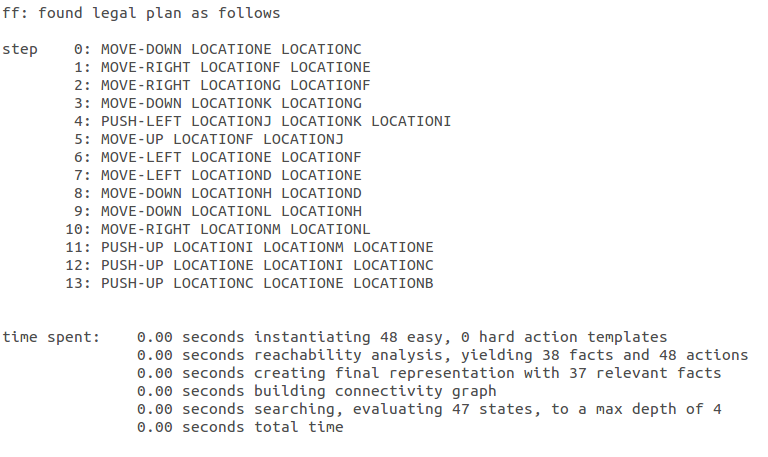
\includegraphics[scale = 0.4]{images/FF_Solution_p2_1}
    \caption{Sokoban Problem 2.1}
  \label{fig_prob2_1}
\end{figure}

\begin{figure}[h!]
  \centering
    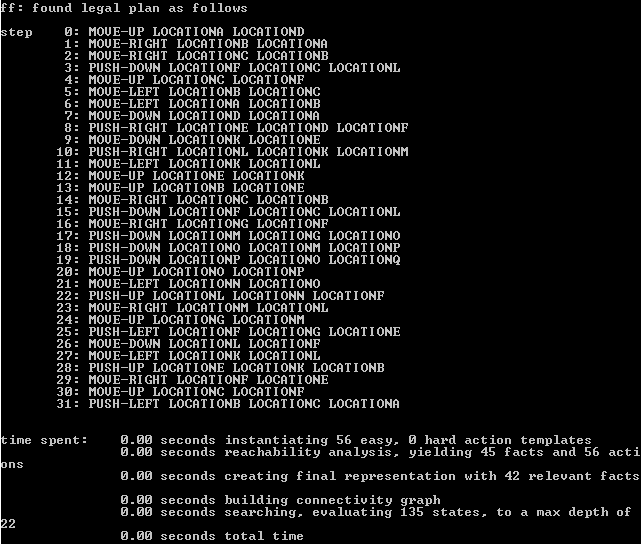
\includegraphics[scale = 0.4]{images/FF_Solution_p2_2}
    \caption{Sokoban Problem 2.2}
  \label{fig_prob2_2}
\end{figure}

\begin{figure} [h!]
\centering
\begin{subfigure}{.5\textwidth}
  \centering
  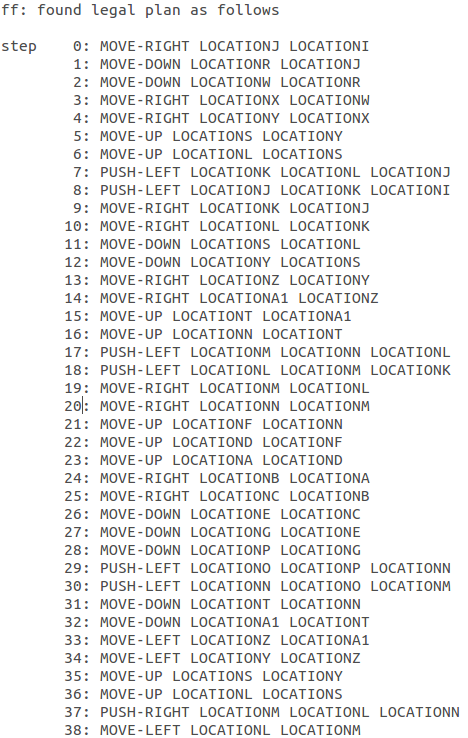
\includegraphics[scale = 0.3]{images/FF_Solution_p2_3_1}
\end{subfigure}%
\begin{subfigure}{.5\textwidth}
  \centering
  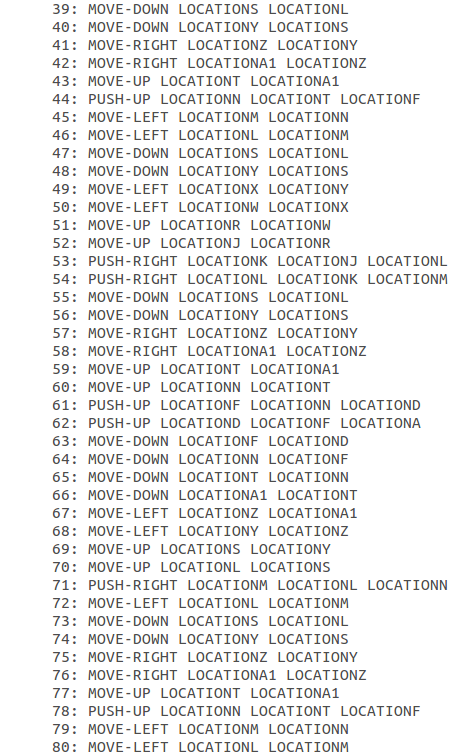
\includegraphics[scale = 0.3]{images/FF_Solution_p2_3_2}
\end{subfigure}\\
\begin{subfigure}{\textwidth}
  \centering
  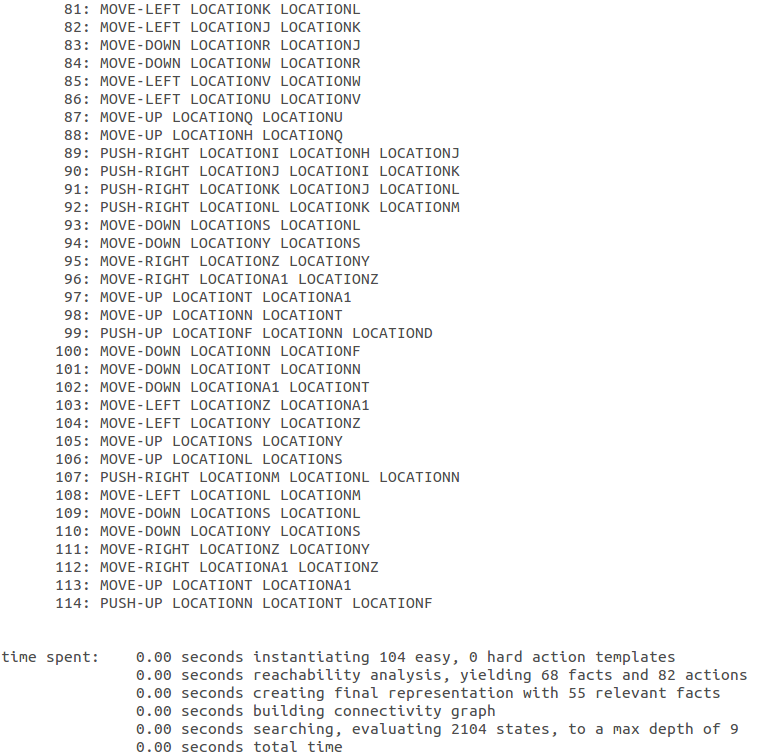
\includegraphics[scale = 0.3]{images/FF_Solution_p2_3_3}
\end{subfigure}%
\caption{Sokoban Problem 2.3}
\label{fig_prob2_3}
\end{figure}

\begin{figure} [h!]
\centering
\begin{subfigure}{.5\textwidth}
  \centering
  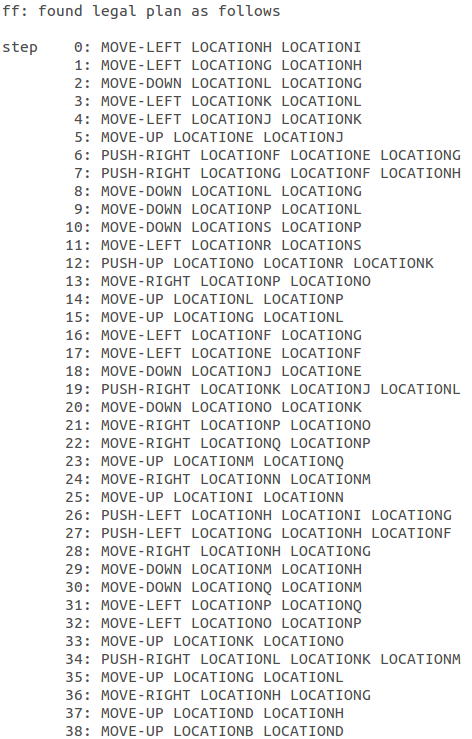
\includegraphics[scale = 0.3]{images/FF_Solution_p2_challenge_1}
\end{subfigure}%
\begin{subfigure}{.5\textwidth}
  \centering
  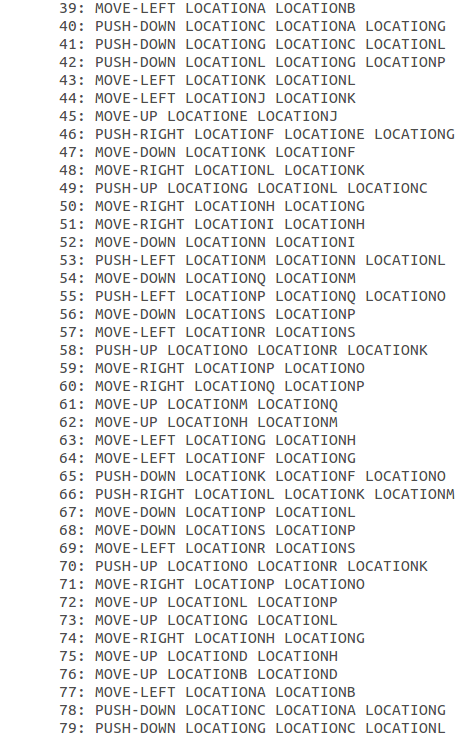
\includegraphics[scale = 0.3]{images/FF_Solution_p2_challenge_2}
\end{subfigure}\\
\begin{subfigure}{\textwidth}
  \centering
  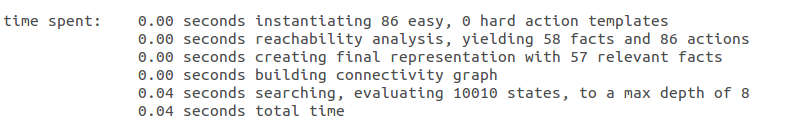
\includegraphics[scale = 0.3]{images/FF_Solution_p2_challenge_3}
\end{subfigure}%
\caption{Sokoban Challenge}
\label{fig_prob2_challenge}
\end{figure}

In order to make the solutions more readable and easier to verify, lets consider that when a robot moves for up, down, right or left direction it will be represented by a lowercase \textbf{u}, \textbf{d}, \textbf{r} or \textbf{l}, respectively. For the push actions of moving the box up, down, right or left, the capital letters \textbf{U}, \textbf{D}, \textbf{R} and \textbf{L} will be used. Thus, the solutions found can be represented as the strings shown below.

\begin{tabular}{ c l }
  &\\
  \textbf{Problem 2.1} & drrdLullddrUUU\\
  &\\
  \textbf{Problem 2.2} & urrDulldRdRluurDrDDDulUruLdlUru\\
  &\\
  \textbf{Problem 2.3} & rddrruuLLrrddrruuLLrruuurrdddLLddlluuRlddrruUllddlluu\\
                       & RRddrruuUUddddlluuRlddrruUllllddlluuRRRRddrruuuddd\\
                       & lluuRlddrruU\\
  &\\
  \textbf{Challenge}   & lldlluRRdddlUruulldRdrruruLLrddlluRuruulDDDlluRdrUrrd\\
                       & LdLdlUrruullDRddlUruuruulDD\\
\end{tabular}

\subsubsection*{2. Compare the performance of two planners on this domain. Which one works better? Does this
make sense, why?}

As an overview, the \textit{FF}'s planner performed better than \textit{Blackbox}. The \textit{FF}'s planner was able to find results for all problems, including challenge, in few seconds. On the other hand, the \textit{Blackbox} only managed to find the results from the first two problems and stopped on the others after using all the hardware resources. These results were expected since, as stated in Section \ref{subsubsec_2}, the \textit{FF}'s planner have a lower asymptotic complexity and use an heuristic function to choose the best option of what expand next. Thus, is more likely to have better time and space complexities than the \textit{Blackbox}.

\subsubsection*{3. Clearly PDDL was not intended for this sort of application. Discuss the challenges in expressing geometric constraints in semantic planning}

While solving this problem is possible to notice that are two approaches. The first one requires a previous knowledge of a solution, and the developer states that a specific box goes to a specific location. The second approach, there is no kind of identification for the boxes, and this is the one we used as a solution. Independently of the approach, the domain contains a grid on which the robot should move. Thus, it is necessary to come up with a way to express when the robot can, or cannot, move between two locations if there is a wall or a box in between. Also, is necessary to express when the robot is allowed to do something, like moving between two empty adjacent squares. Thus, all these logic expressions were used to represent geometric constraints like collisions between the robot and the walls or boxes.

\subsubsection*{4. In many cases, geometric and dynamic planning are insufficient to describe a domain. Give
an example of a problem that is best suited for semantic (classical) planning. Explain why a
semantic representation would be desirable}

The classical planners have a variety of best suited problems, like in logistics, manofacturing, and management. One example is the DART system used for military logistics. Logistics are better expressed by a set of logical expressions to specify complex operations not related to the kinect motion.

%------------------------------------End of Problem 2 -------------------------------------------------%

\section{Project Part II: Sokoban Planner}
%Assigned to James and Stango%
\subsection{Questions}
\subsubsection*{1. Give successful plans from your planner on the Sokoban problems in Figure \ref{fig2} and any others}
\subsubsection*{2. Compare the performance of your planner to the PDDL planners you used in the previous
problem. Which was faster? Why?}
\subsubsection*{3. Prove that your planner was complete. Your instructor has a math background: a proof ``is
a convincing argument.'' Make sure you address each aspect of completeness and why your
planner satisfies it. Pictures are always welcome.}
\subsubsection*{4. What methods did you use to speed up the planning? Give a short description of each method
and explain why it did or didn't help on each relevant problem}

%---------------------------------End of Problem 3 ----------------------------------------------------%

\section{Post-Project: Towers of Hanoi Revisited}
%Assigned to Arvind%
Constructing a PDDL representation for the N-disk towers of hanoi is pretty simple by utilizing the following simple structures, for initializing the problem state
\begin{enumerate}
\item Each disk labeled $D_i$ is smaller than a disk labeled $D_{i+1}$. That is \texttt{(smaller $d_i$ $d_{i+1}$)}.
\item Every disk is smaller than each of the three poles (by definition).
\item The smallest disk (i.e., D1), and the two other poles (P1 and P2) are clear.
\item Every disk $D_i$ is \emph{on} the disk $D_{i+1}$. The largest disk D10, is \emph{on} the pole P3.
\item Every element $D_i$ is a disk
\end{enumerate}
The goal state is simply a conjunction (\textsc{And}-ing) of all the states mentioned in Step 4 above, except that the largest disk D10, is \emph{on} the pole P1.

The corresponding PDDL representations for the 6 disk and 10 disk towers of hanoi problem are present in the files ``hanoi-6.pddl'' and ``hanoi-10.pddl''.

Both \textbf{FF} and \textbf{Blackbox} planners were applied onto the PDDL representations, however only \textit{FF} was able to produce valid plans for the 6 disk and 10 disk problem. \textit{Blackbox} was unable to produce any results, due to relatively large nature of the state-space (I halted execution after 1 minute since the blackbox executable started running).

\subsection{Questions}
\subsubsection*{1. Give successful plans from at least one planner with 6 and 10 disks}
The plan for the towers of hanoi problem with 6 disks, generated by \textit{FF} is shown in Figure \ref{plan6}.

\begin{figure}[h!]
\centering
\begin{subfigure}{.5\textwidth}
  \centering
  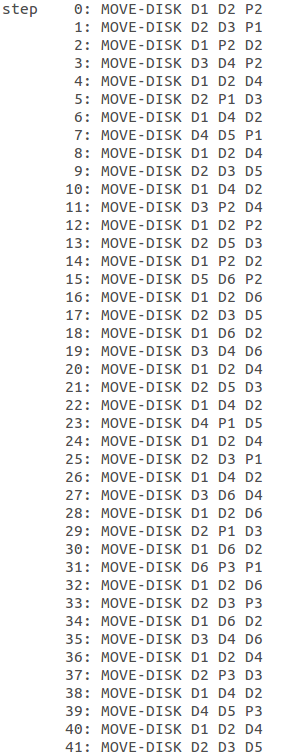
\includegraphics[scale = 0.3]{images/hanoi-6_1}
\end{subfigure}%
\begin{subfigure}{.5\textwidth}
  \centering
  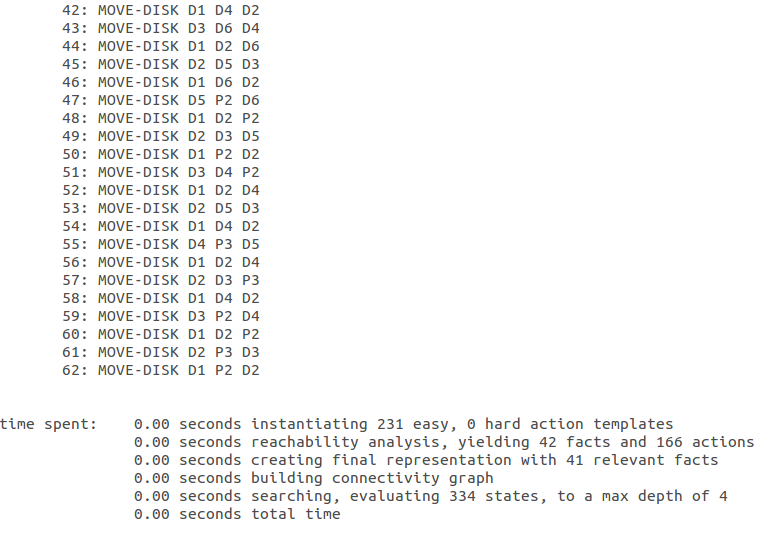
\includegraphics[scale = 0.3]{images/hanoi-6_2}
\end{subfigure}%
\caption{Plan for Towers of Hanoi with 6 disks}
\label{plan6}
\end{figure}

Clearly it has $2^6 - 1$ = 63 steps in the plan. Now the problem with 10 disks will have a plan of $2^{10} - 1$ = 1023 steps. The \textit{FF} planner produces a valid plan with 1023 steps, but for the lack of space it is not produced here. The plan is present under the resources directory as ``hanoi-10-solutions''.

\subsubsection*{2. Do you notice anything about the structure of the plans? Can you use this to increase the
efficiency of planning for Towers of Hanoi? Explain}
One observation from the three plans generated (3, 6 and 10 disks) is that whenever there are odd number of initial disks, then the top most disk is moved onto the ``destination'' pole, and when there are even number of initial disks, then the top most disk is moved onto the ``middle'' pole.

Another noticeable aspect of the problem is that the towers of hanoi can be viewed as a simple recursive problem of moving the smaller $n-1$ disks from $P3$ to $P2$ then moving the largest disk from $P3$ to $P1$ followed by moving the $n-1$ disks from $P2$ to $P1$. This can be empirically verified - at every $(2^N - 1)^{th}$ step, if the initial number of disks $n$ are odd, then there will be $N-1$ disks on P2 and largest disk will be on P1. If the initial number of disks $n$ are even, then there will be $N-1$ disks on $P3$ and the largest will be on $P2$. Of course here, $0<N<=n$.

Thus the entire plan can be represented recursively (and efficiently) as: 
\begin{algorithm}
  \caption{Towers of Hanoi recursive definition}
  \begin{algorithmic}[1]
    \Function{Hanoi-Solver}{$N, P3, P2, P1$}
    \Comment{Move N disks from P3 to P1 (using P2 as intermediate)}
		\State \Call{Hanoi-Solver}{$N-1, P3, P1, P2$}
		\State \Call{Move}{$1, P3, P1$} \Comment{Move the largest disk from P3 to P1}
	  	\State \Call{Hanoi-Solver}{$N-1, P2, P3, P1$}
    \EndFunction
  \end{algorithmic}
\end{algorithm}

Thus this is a bottom-up approach in constructing a plan. All one needs to define are the ``macro'' propositions \textsc{Hanoi-Solver} and \textsc{Move} (which is applied when there is just the largest disk remaining on $P3$). The planner can then use this base condition (a.k.a ``macro'' proposition) and basically ``un-wind'' the call stack to generate sub-plans. The correct plan is then obtained by simply reversing the ``popped'' elements of the call stack.


\subsubsection*{3. In a paragraph or two, explain a general planning strategy that would take advantage of
problem structure. Make sure your strategy applies to problems other than Towers of Hanoi.
Would such a planner still be complete?}

A general recursive algorithm takes advantage of whenever there is a possibility of breaking down a problem into multiple smaller, but similarly structured problems, each if solved (and possibly in parallel if there is sufficient independence) can be ``combined'' to get the solution to the original problem. The generic recursive algorithm is:

\begin{algorithm}
  \caption{Recursive Planner}
  \begin{algorithmic}[1]
    \Function{Recursive-Planner}{$Prob_N$}
    \Comment{Solve a sub-problem}
    		\If{Some Terminal Condition}
			\State \Call{Terminal-Operation}{$Prob_1$} \Comment{Some constant terminal operation}
		\EndIf
		\State \Call{Recursive-Planner}{$Subset(Prob_N)$}
    \EndFunction
  \end{algorithmic}
\end{algorithm}

There are a whole class of problems to which a recursive planner can be applied. For instance, this algorithm can be used in large scale map navigation problems, where loading an entire terrain in one go may be memory prohibitive.

There are two conditions for a planner to be complete,
\begin{enumerate}
\item \textbf{Produces a plan if there is one}: The recursive planner relies on all the sub-goals to complete their execution (or the recursion stack to be empty). So in case all the sub-goals reach their respective terminating condition, then all of them will reach completion (this is from an execution standpoint - different from the notion of completeness). If all the individual problems finish, then the top-level problem, which is basically a composition of these sub-problems will also produce a valid plan.

However, it is possible that even though the entire problem has a solution, one of the sub-problems may never reach completion -- this would cause the original problem to not produce a plan. Hence it cannot always be guaranteed that the planner produces a plan if there is a valid one.

\item \textbf{Reports that there is no plan if there is none}: The same sub-problem non-termination issue exists here as well. In case one of the sub-problems gets ``stuck'', there is no way for the original problem to terminate reporting that there is no plan. 
\end{enumerate}

However, if some sort of a terminating ``\textit{parameter}'' can be used to force the sub-problems to halt/report no solution. In such a case the ``stack overflow'' issue will be resolved and both the conditions of completeness will be met. Basically, we need to ensure that the sub-problems will be forcibly terminated which will ensure that the main problem will always terminate as well!

%----------------------------------End of Problem 4 ----------------------------------------------------%

\bibliographystyle{unsrt}
\bibliography{myrefs}
\end{document}